\documentclass{article}

\usepackage{listings}
\usepackage{color}
\usepackage{graphicx}
\usepackage{float}
\usepackage{amsmath}
\usepackage{subfig}
\usepackage{cite}
\usepackage{url}

\begin{document}

\title{Image Analysis - TP3 - Corner detection}

\author{Jander Nascimento, 
\and Raquel Oliveira}

\maketitle

\section{Gradient Images}
	
	\subsection{Horizontal and vertical gradient}

	The gradient is created based on a vector that points to the highest rate of change in the magnitude, and can be represented as in the Formula \ref{eq:gradient}. 

\begin{equation}
\bigtriangledown f = \begin{pmatrix}
\frac{\partial f}{\partial x} = M_x\\ 
\frac{\partial f}{\partial y} = M_y
\end{pmatrix}
\label{eq:gradient}
\end{equation}

The gradient can be reached in several manners, the performance and accuracy contraints may dictate which method best fits. 

For this specific project, the method adopted was a kernel convolution with the sobel operator, that is an approximation of the integral. 

The both sobel operators, horizontal and vertical, can be seen in the the Table \ref{tab:sobelx} and \ref{tab:sobely}. Each of them are applied individually to the source image to produce different images.

\begin{figure}
  \begin{center}
  \begin{tabular}{ | c | c | c | }
    \hline
    -1 & -2 & -1 \\ \hline
    0 & 0 & 0 \\ \hline
    1 & 2 & 1 \\
    \hline
  \end{tabular}
  \end{center}
  \caption{$G_y$: Horizontal sobel operator\label{tab:sobely}}
\end{figure}

\begin{figure}
  \begin{center}
  \begin{tabular}{ | c | c | c | }
    \hline
    -1 & 0 & 1 \\ \hline
    -2 & 0 & 2 \\ \hline
    -1 & 0 & 1 \\
    \hline
  \end{tabular}
  \end{center}
  \caption{$G_x$: Vertical Sobel operator\label{tab:sobelx}}
\end{figure}


There exist several filters that can be used to find the gradient. e.g: sobel and prewitt. Here was used the sobel operator to reach the results.

The sobel operator is a pair of kernels (one for vertical and one horizontal edges detection) which can be convoluted which the image to obtain their respective gradient.

In the Figure \ref{fig:gradient} we can see the result of the horizontal and vertical gradient.

	\begin{figure}[H]
	\centering
	\subfloat[Original Image]{\label{fig:original}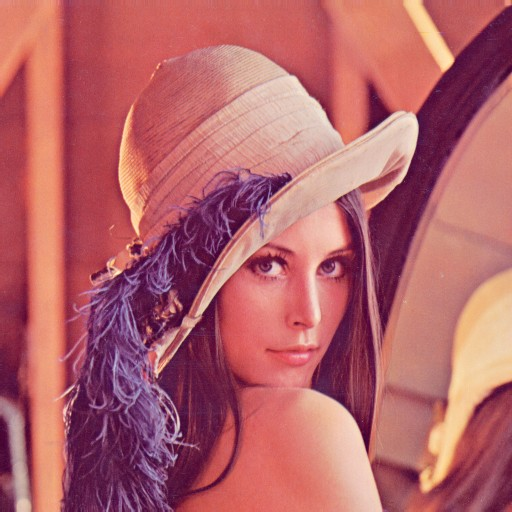
\includegraphics[width=0.3\textwidth]{../lena}}                
	\subfloat[Horizontal Gradient]{\label{fig:horizontal}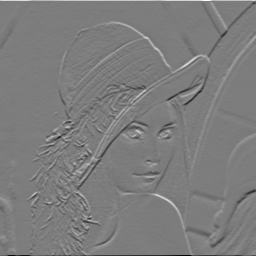
\includegraphics[width=0.3\textwidth]{../img/lena_gradienty}}                
	\subfloat[Vertical Gradient]{\label{fig:vertical}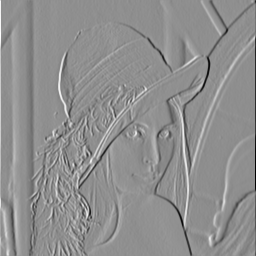
\includegraphics[width=0.3\textwidth]{../img/lena_gradientx}}                
	\caption{Gradient}
	\label{fig:gradient}
	\end{figure}


\section{Gradient Norm}

Gradient norm is the mathematical representation of the vector. This can be reached through one of the two Equations \ref{equa:norm1} or \ref{equa:norm2}.

The result of the Gradient norm can be seen in the Figure \ref{fig:norm_gradient}. 

\begin{figure}[H]
	\centering
	\subfloat[Horizontal Gradient]{\label{fig:norm_horizontal}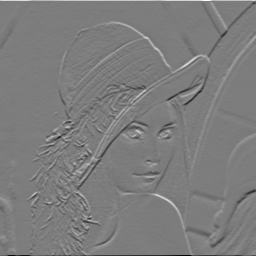
\includegraphics[width=0.3\textwidth]{../img/lena_gradienty}}                
	\subfloat[Vertical Gradient]{\label{fig:norm_vertical}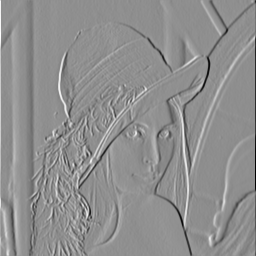
\includegraphics[width=0.3\textwidth]{../img/lena_gradientx}}                
	\subfloat[Gradient norm]{\label{fig:norm}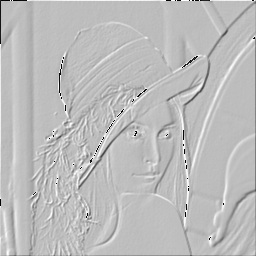
\includegraphics[width=0.3\textwidth]{../img/lena_gradientxy}}                
	\caption{Gradient}
	\label{fig:norm_gradient}
\end{figure}

%\begin{equation}
%magn(\bigtriangledown f) = \sqrt{M_x^{2}+M_y^{2}}\approx \left | M_x \right |+\left | M_y \right |
%\label{equa:norm}
%\end{equation}

\begin{equation}
G = \sqrt{G_x^{2}+G_y^{2}}
\label{equa:norm1}
\end{equation}

\begin{equation}
G = | G_x | + | G_y |
\label{equa:norm2}
\end{equation}

Both Equations are valid, but once more the computational costs differs from one to another.

\section{Corner Detection}




\end{document}


